\chapter{Transport Mechanisms}

\section{Viscosity and Demonstrating Momentum Transport}

Viscosity is a measure of a fluid's tendency to resist flow. Generally we represent the viscosity of a fluid by $\mu$. 

Before describing the properties of viscosity and how it changes, let us observe qualitatively how a viscous fluid behaves when we try to make it flow under some forces.

Given below is a simple, illustrative situation:

\begin{figure}[h]
    \centering
    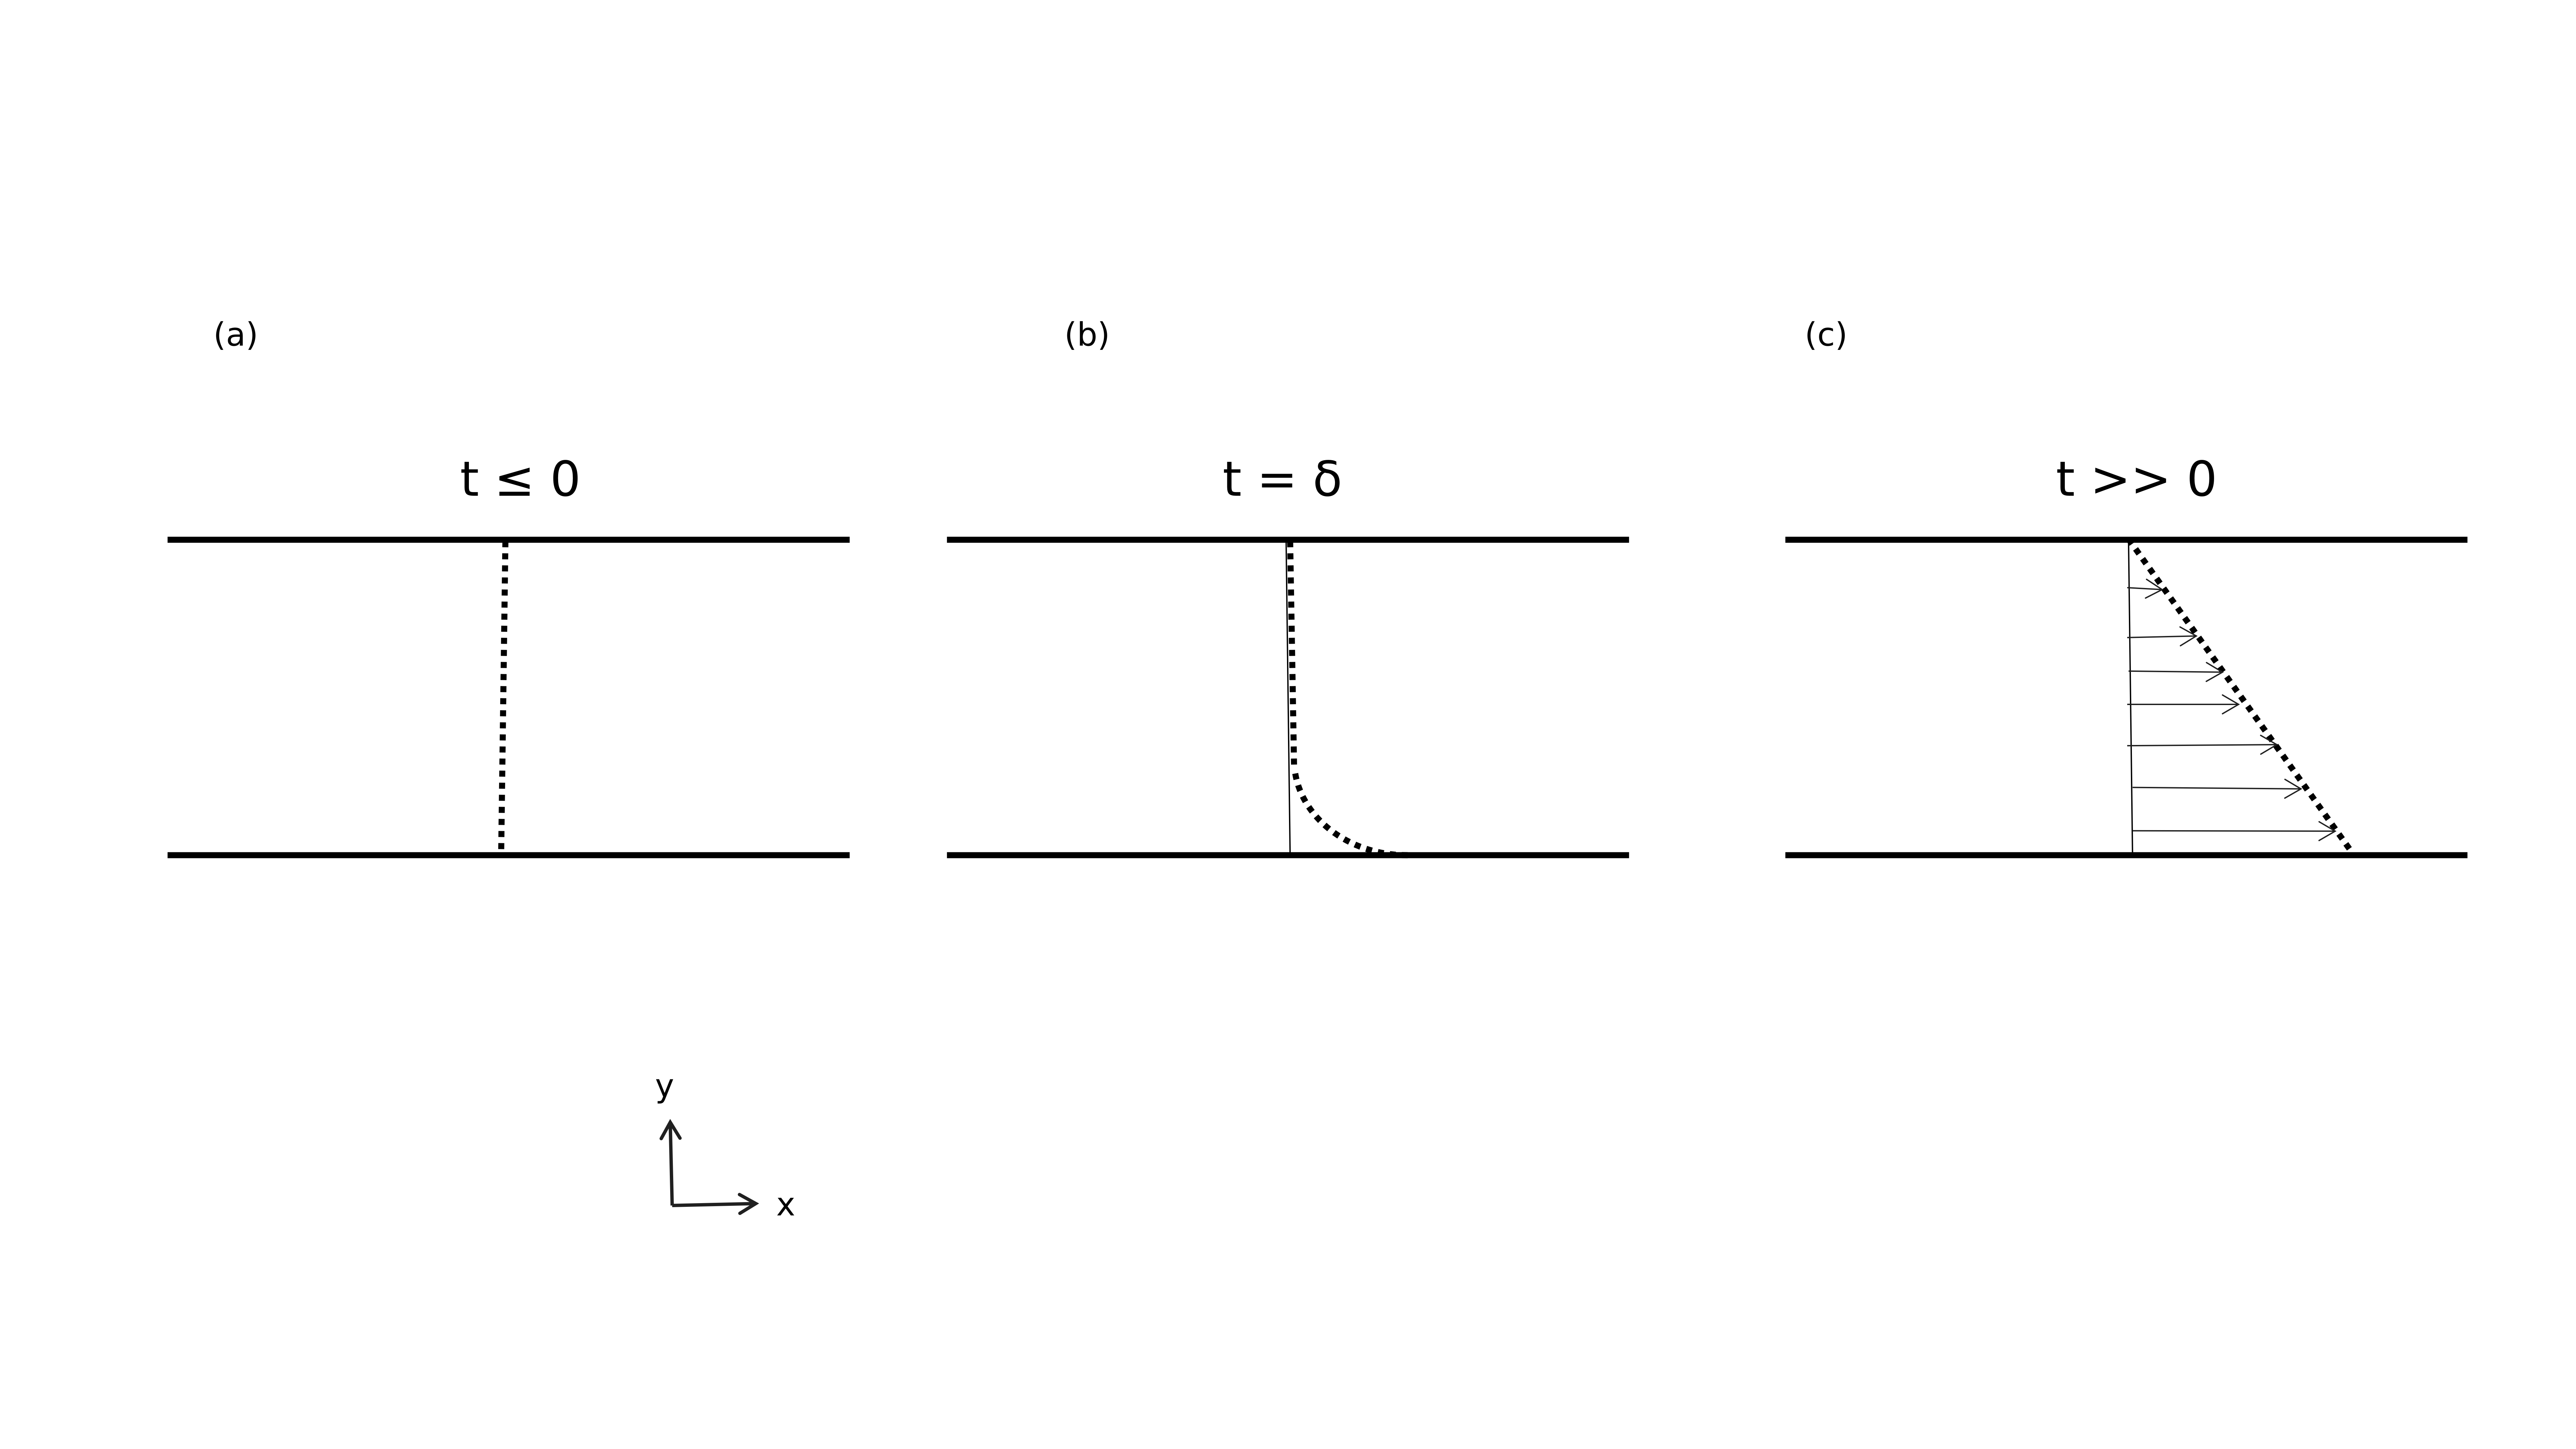
\includegraphics[scale=0.1]{figure1_01}
    \caption{Fluid between 2 plates}
\end{figure}

\begin{itemize}
    \item Consider two parallel plates : one placed at y = 0 and the other placed at y = Y as shown in figure 1.1, with a static fluid between them. Here we assume these plates are basically infinitely long and wide so that the fluid doesn't move. Figure 1.1(a) shows how the fluid velocity is 0 at every point between the two plates. 

    \item Now, let us see what happens when we begin to translate the bottom plate to the right. Assuming there is no slip between the fluid and the plate, i.e. that the fluid that comes into contact with the solid is "stuck" to it. At the molecular scale, this is because we consider adhesive forces of attraction between molecules of the fluid and the solid are stronger than the cohesive forces of attraction among the molecules of the fluid themselves. So when we move the bottom plate, the molecules in contact with it start to move along. Figure 1.1(b) describes a snapshot of the system where the molecules "stuck" to the plate have just started to move but the molecules above them haven't been impacted yet.

    \item Over time, the fluid layers begin to pull each other and due to this, momentum gets imparted along the y direction. Figure 1.1(c) showcases the steady-state velocity profile of the fluid. Again, at the top plate the fluid doesn't move since the molecules are assumed to be "stuck" to the plate. 
\end{itemize}

We began our observation of the transport of momentum by seeing how the fluid molecules in contact with the lower plate are dragged along. But it is important to note that the plate is also being dragged by the fluid! So we have to apply some force F to keep the plate going. How much does the fluid drag the plate?

$$\frac{F}{A} = \mu \frac{V}{Y}$$

This can be extended to looking at the force per unit area that each differential "slice" of fluid experiences:


\begin{empheq}[box=\fbox]{align}
\tau_{yx} = -\mu \frac{dv_{x}}{dy}
\end{empheq}

This is a very important equation and is referred to as Newton's Law of Viscosity.

Some key points to note about Newton's Law of Viscosity:

\begin{itemize}
    \item This equation showcases the transport of the $x$ component of momentum in the y direction.

    \item $\tau_{xy} = F/A$ here refers to the force in $x$ direction per unit area perpendicular to $y$ direction. This quantity is the flux of x-component of momentum in the y direction. 

    \item The law applies to other directions as well. If we consider a pair of \textbf{unequal} directions i, j, we can generalise this and state that $$\tau_{ij} = -\mu \frac{dv_{j}}{di}$$.

    \item If i = j, then we get (for example i = j = x) $$\tau_{xx} = -2 \mu \frac{dv_{x}}{dx}$$.

    \item Here we consider $\mu$ to be invariant of the directions (we don't say $\mu_{xy}$ etc.). This makes an inherent assumption about the isotropy of the fluid, i.e. that the properties of the fluid don't vary in different directions. This is not necessarily true in certain complex fluids and polymer solutions. 
\end{itemize}

Note that it's very easy to see how $\tau$ refers to "momentum flux" by just looking at dimensions. Force is (mass).(acceleration) = (mass).(velocity/time) = (momentum/time) or rate of momentum. Now Force/Area is just flux of momentum, simple!

\textbf{It is very important to remember that $\tau_{yx}$ is the flux of "x-momentum in y direction"}. It is easy to flip the order and make a mistake, so be careful.

\subsection*{Some more points on viscosity}

\begin{itemize}
    \item The dimensions of $\mu$ is (pressure).(time) and hence the SI unit is pascal-second or (Pa)(s). However a more convenient unit for engineering problems is centipoise (cP). Keep in mind that $1 cP = 10^{-3} Pa.s$. Water has a viscosity of about 1 cP at room temperature.

    \item At low densities 
        \SubItem{\textbf{Gases:} Viscosity increases with temperature}
        \SubItem{\textbf{Liquids:} Viscosity decreases with temperature}

    \item Kinematic viscosity can be defined as $$\nu = \frac{\mu}{\rho}$$

    \item A useful quantity that describes the flow properties of a fluid is the Reynolds' number (Re). It is given by : $$Re = \frac{\rho v d}{\mu}$$ where $v$ is a characteristic velocity of the system and $d$ is a characteristic length. It represents the ratio of inertial forces to viscous forces in a fluid system.
\end{itemize}

\section{Mechanisms of Momentum Transport}

\subsection{Vectors and Tensors in Transport}

Some important notation:


\begin{itemize}

    \item \textbf{v} is the velocity vector.

    \item $v_{x}$ is the x component of the velocity vector which is a function: $v_{x} (x, y, z, t)$.

    \item The unit vectors are denoted by \textbf{$\delta_{x}$, $\delta_{y}$, $\delta_{z}$} in x, y, z directions.

    \item Tensors are multilinear objects relating vectors. In the case of fluids, we are mainly concerned with "order 2" tensors, which can be depicted similar to matrices. For example, $\tau$ is an order two tensor whose components are $\tau_{ij}$.

$$\begin{bmatrix}  

    \tau_{xx} & \tau_{xy} & \tau_{xz} \\
    \tau_{yx} & \tau_{yy} & \tau_{yz} \\
    \tau_{zx} & \tau_{zy} & \tau_{zz} \\
    
\end{bmatrix}$$

    \item This is a 9-component tensor. The diagonal components represent normal stresses while other terms are shear stresses.

    \item We can also consider one component out of our tensors: which then becomes a vector. For example if we take the x component of $\tau$, we have $\tau_{x}$ which is a vector.

\end{itemize}


\subsection{Molecular Momentum Transport}

Molecular transport of momentum is the extent of momentum transport that can be attributed to molecular forces. In figure 2, we take a differential fluid element and observe the forces. First let us only consider forces acting in the x-direction, for simplicity. For this, we observe a plane perpendicular to the x-axis (or parallel to the yz plane). For this plane there are 2 forces :

\begin{itemize}
    \item Viscous force $\tau_{x}$ which has three components.

    \item Pressure force $P \delta{x}$. Note again that $\delta_{x}$ is the x-direction unit vector. 
\end{itemize}


\begin{figure}[h]
    \centering
    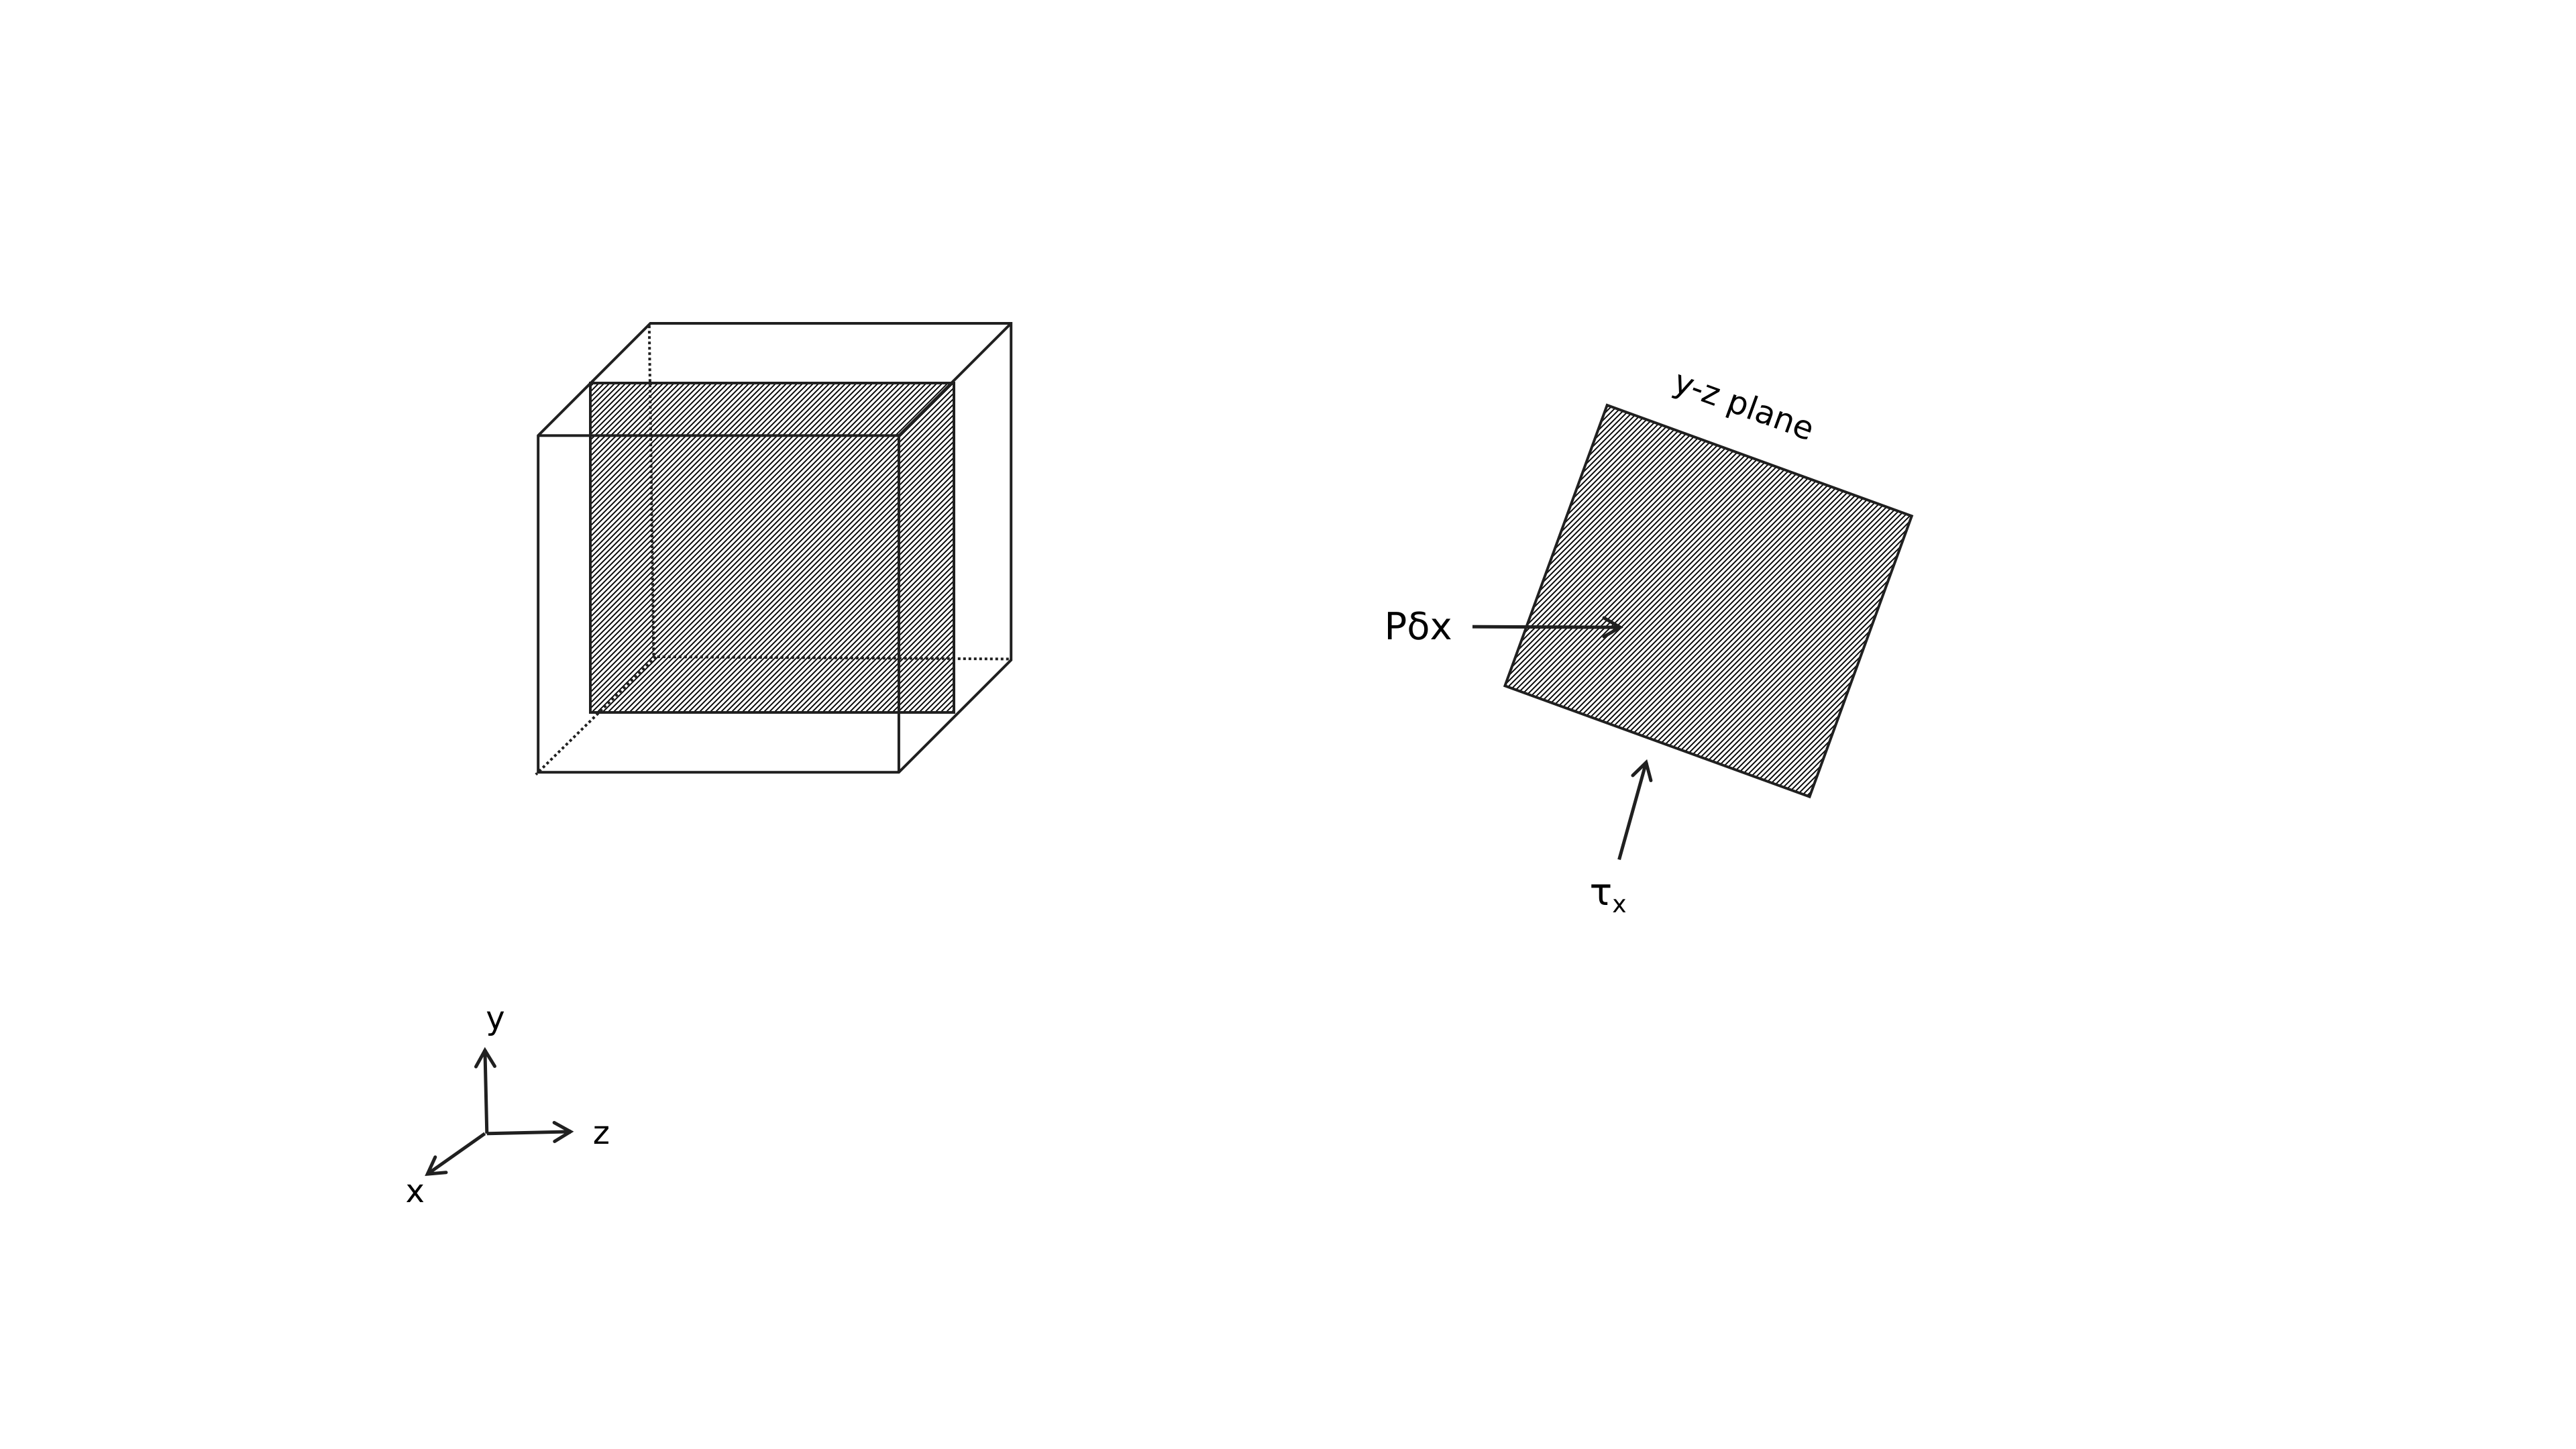
\includegraphics[scale=0.1]{figure2_01}
    \caption{Forces on a fluid element}
\end{figure}


In the absence of a velocity gradient, there are no viscous forces since fluid elements move together but pressure forces still act.

Hence, there are 6 forces tugging this fluid element : 3 pressure forces $P \delta{x}, P \delta{y}, P \delta{z}$ and 3 viscous forces $\tau_{x}, \tau_{y}, \tau_{z}$.

Now, we can define a \textbf{molecular momentum flux} ($\pi$) which gives us the flux of momentum due to molecular forces. We need it to incorporate the pressure term and the viscous term. As described in Figure 2, let us only consider this molecular momentum flux across a plane perpendicular to the x axis.

The viscous terms are easy to incorporate. $\pi_{xx}$ would have the term $\tau_{xx}$, $\pi_{xy}$ would incorporate $\tau_{xy}$ and so on. The pressure term meanwhile only has one direction (x), so we expect it to appear only in the $\pi_{xx}$ expression.

In summary :

$$\pi_{xx} = P + \tau_{xx}$$

$$\pi_{xy} = \tau_{xy}$$

$$\pi_{xz} = \tau_{xz}$$


Similar expressions can be written for $\pi_{y}$ and $\pi_{z}$. For $\pi_{y}$ the pressure term will appear in $\pi_{yy}$ only and for $\pi_{z}$ it'll appear only in $\pi_{zz}$.

If we wanted to condense our expression for $\pi$ into one terse statement, we can write it as such :


\begin{empheq}[box=\fbox]{align}
    \pi_{ij} = P \delta_{ij} + \tau_{ij}
\end{empheq}

Here $\delta_{ij}$ is the Kronecker delta function (which has a value of 1 when i = j and 0 otherwise). \textbf{$\pi_{ij}$ is the flux of j-momentum in the i direction, from a region of less i to greater i.} $\pi$ is again a tensor with the diagonal terms being normal stresses and other components being shear stresses.


\subsection{Convective Momentum Transport}

Apart from molecular forces, momentum can also be transported by bulk flow of fluid. This is called "convective momentum transport". 


\begin{figure}[h]
    \centering
    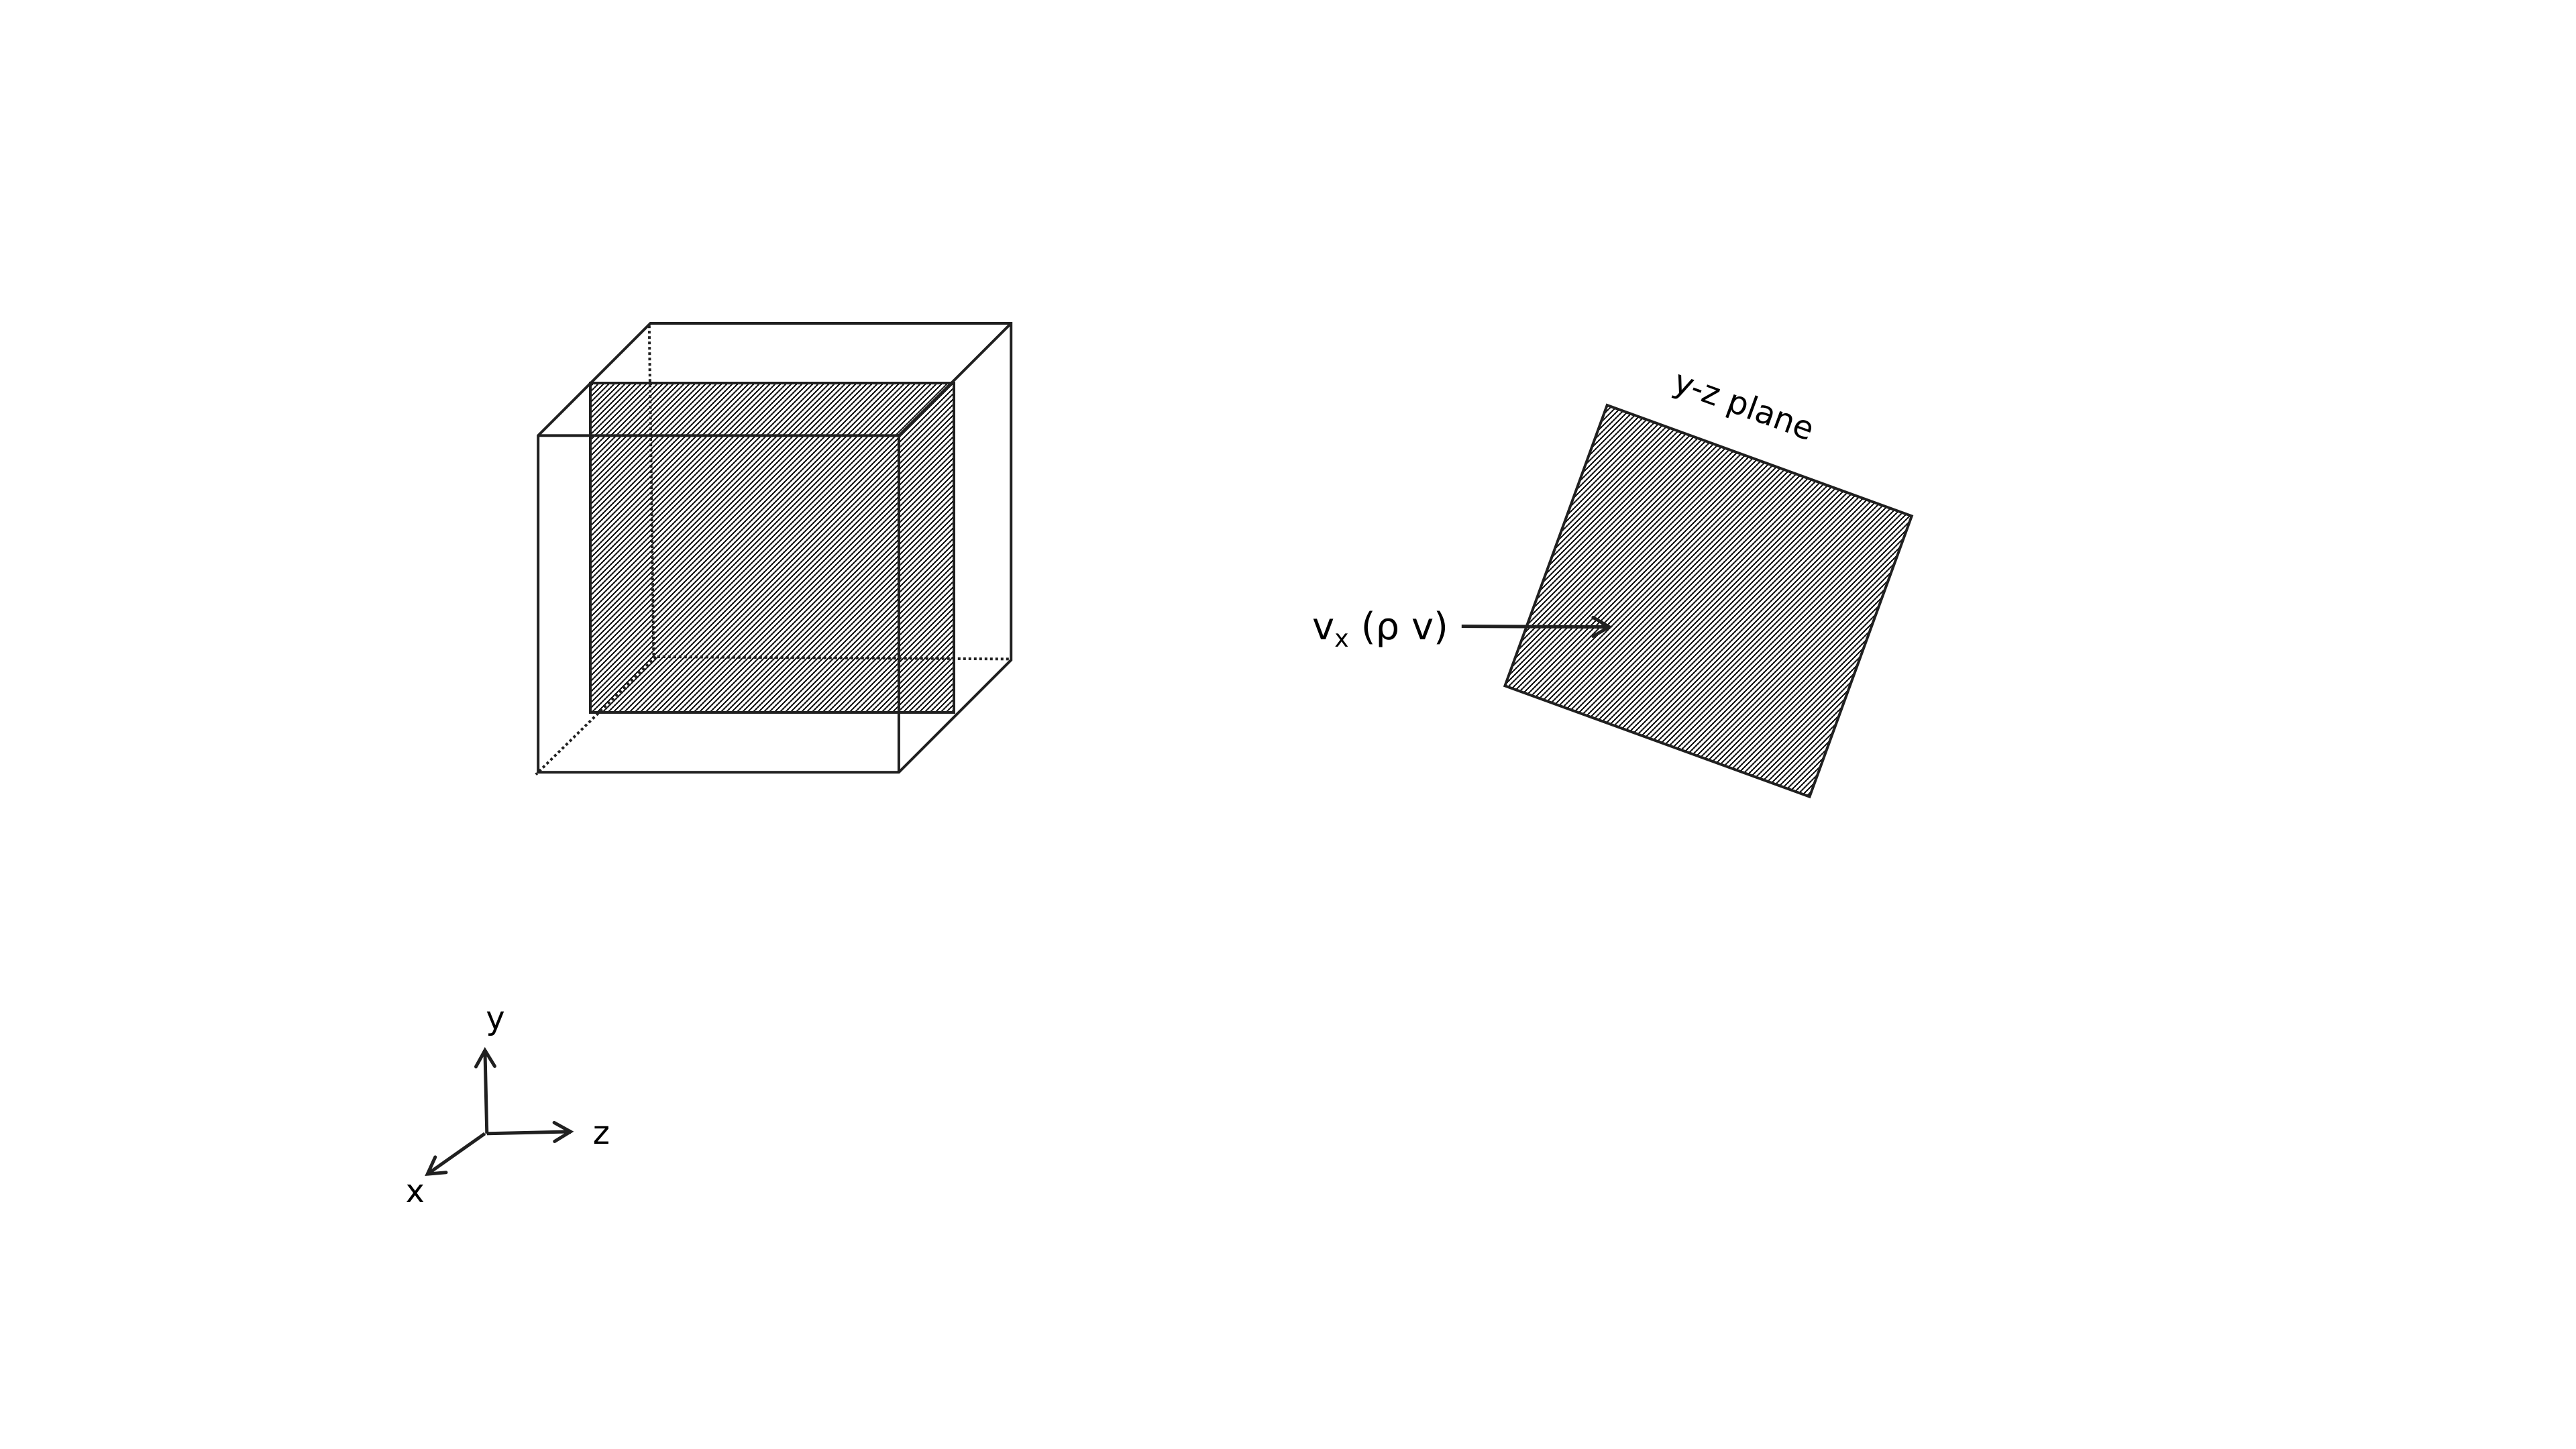
\includegraphics[scale=0.1]{figure2_02}
    \caption{Convective Momentum Transport}
\end{figure}

In figure 3, we see the same fluid element again, but this time let us only consider the convective terms. The volume rate of fluid flow across the shaded area is $v_{x}$. And it carries a momentum vector \textbf{$\rho$ v} (here we look at momentum per unit volume). Hence the momentum flux is simply $v_{x} \rho$ \textbf{v}. This quantity is the convective momentum flux across a plane perpendicular to the x-axis.

The tensor for convective momentum transport can be represented as $\rho$ \textbf{v v}. As in the case of molecular momentum flux tensor, this is also a 9-component tensor. 


\subsubsection*{Combined Momentum Flux}

To denote the total momentum flux experienced by a fluid in various directions, we use the tensor $\phi$. It is the sum of molecular and convective momentum fluxes.

\begin{empheq}[box=\fbox]{align}
    \phi = \pi + \rho \textbf{v v}
\end{empheq}

Consider some example components of this tensor:

$$\phi_{zz} = P + \tau_{zz} + \rho v_{z} v_{z}$$

$$\phi_{xy} = \tau_{xy} + \rho v_{x} v_{y}$$



\section*{Questions}

\begin{enumerate}
    \item Consider a set of vectors {\textbf{$v_{i}$}}, where all the vectors are orthogonal (perpendicular) to each other. We want to develop a terse notation to show this orthogonality. Which of these are suitable?

        (a) $v_{i} \cdot v_{j} = |v|^{2}$

        (b) $v_{i} \cdot v_{j} = |v|^{2} \delta_{ij}$

        (c) $v_{i} - v_{j} = (\delta_{x} - \delta_{y})(|v_{i}| - |v_{j}|)$ 

        (d) $v_{i} + v_{j} = (\delta_{x} + \delta_{y})(|v_{i}| + |v_{j}|)$

    \item Two infinite parallel plates, separated by 1m have a viscous static fluid of viscosity 1 cP between them. The top plate is translated to the left with a velocity of 5 $m s^{-1}$ and the bottom plate is translated to the right by 6 $m s^{-1}$. After reaching steady-state, what is the velocity of a fluid element half-way between the plates? Is that fluid element moving to the right or left?

    \item A boat with sophisticated measurement machinery is going around a lake on a windy day and measuring stresses. The velocity of the lakewater at a point (x, y) is given by $v_{x}(x, y), v_{y}(x, y)$, where $v_{x}(x, y) = A e^{-(x+y)}$, $v_{y}(x,y) = B \frac{x + y}{xy}$ Write the components of the viscous stress tensor for this system. 

    \item Verify that the per-volume momentum $\rho$ \textbf{v} when multiplied by velocity \textbf{v} does in fact give a momentum flux quantity.

\end{enumerate}


\section{Thermal Conductivity and Demonstrating Energy Transport}

In a similar manner to how we saw the qualitative behaviour of a viscous fluid between two solid plates, we shall demonstrate the behaviour of thermal conductivity of a solid slab between two plates. 


\begin{figure}[h]
    \centering
    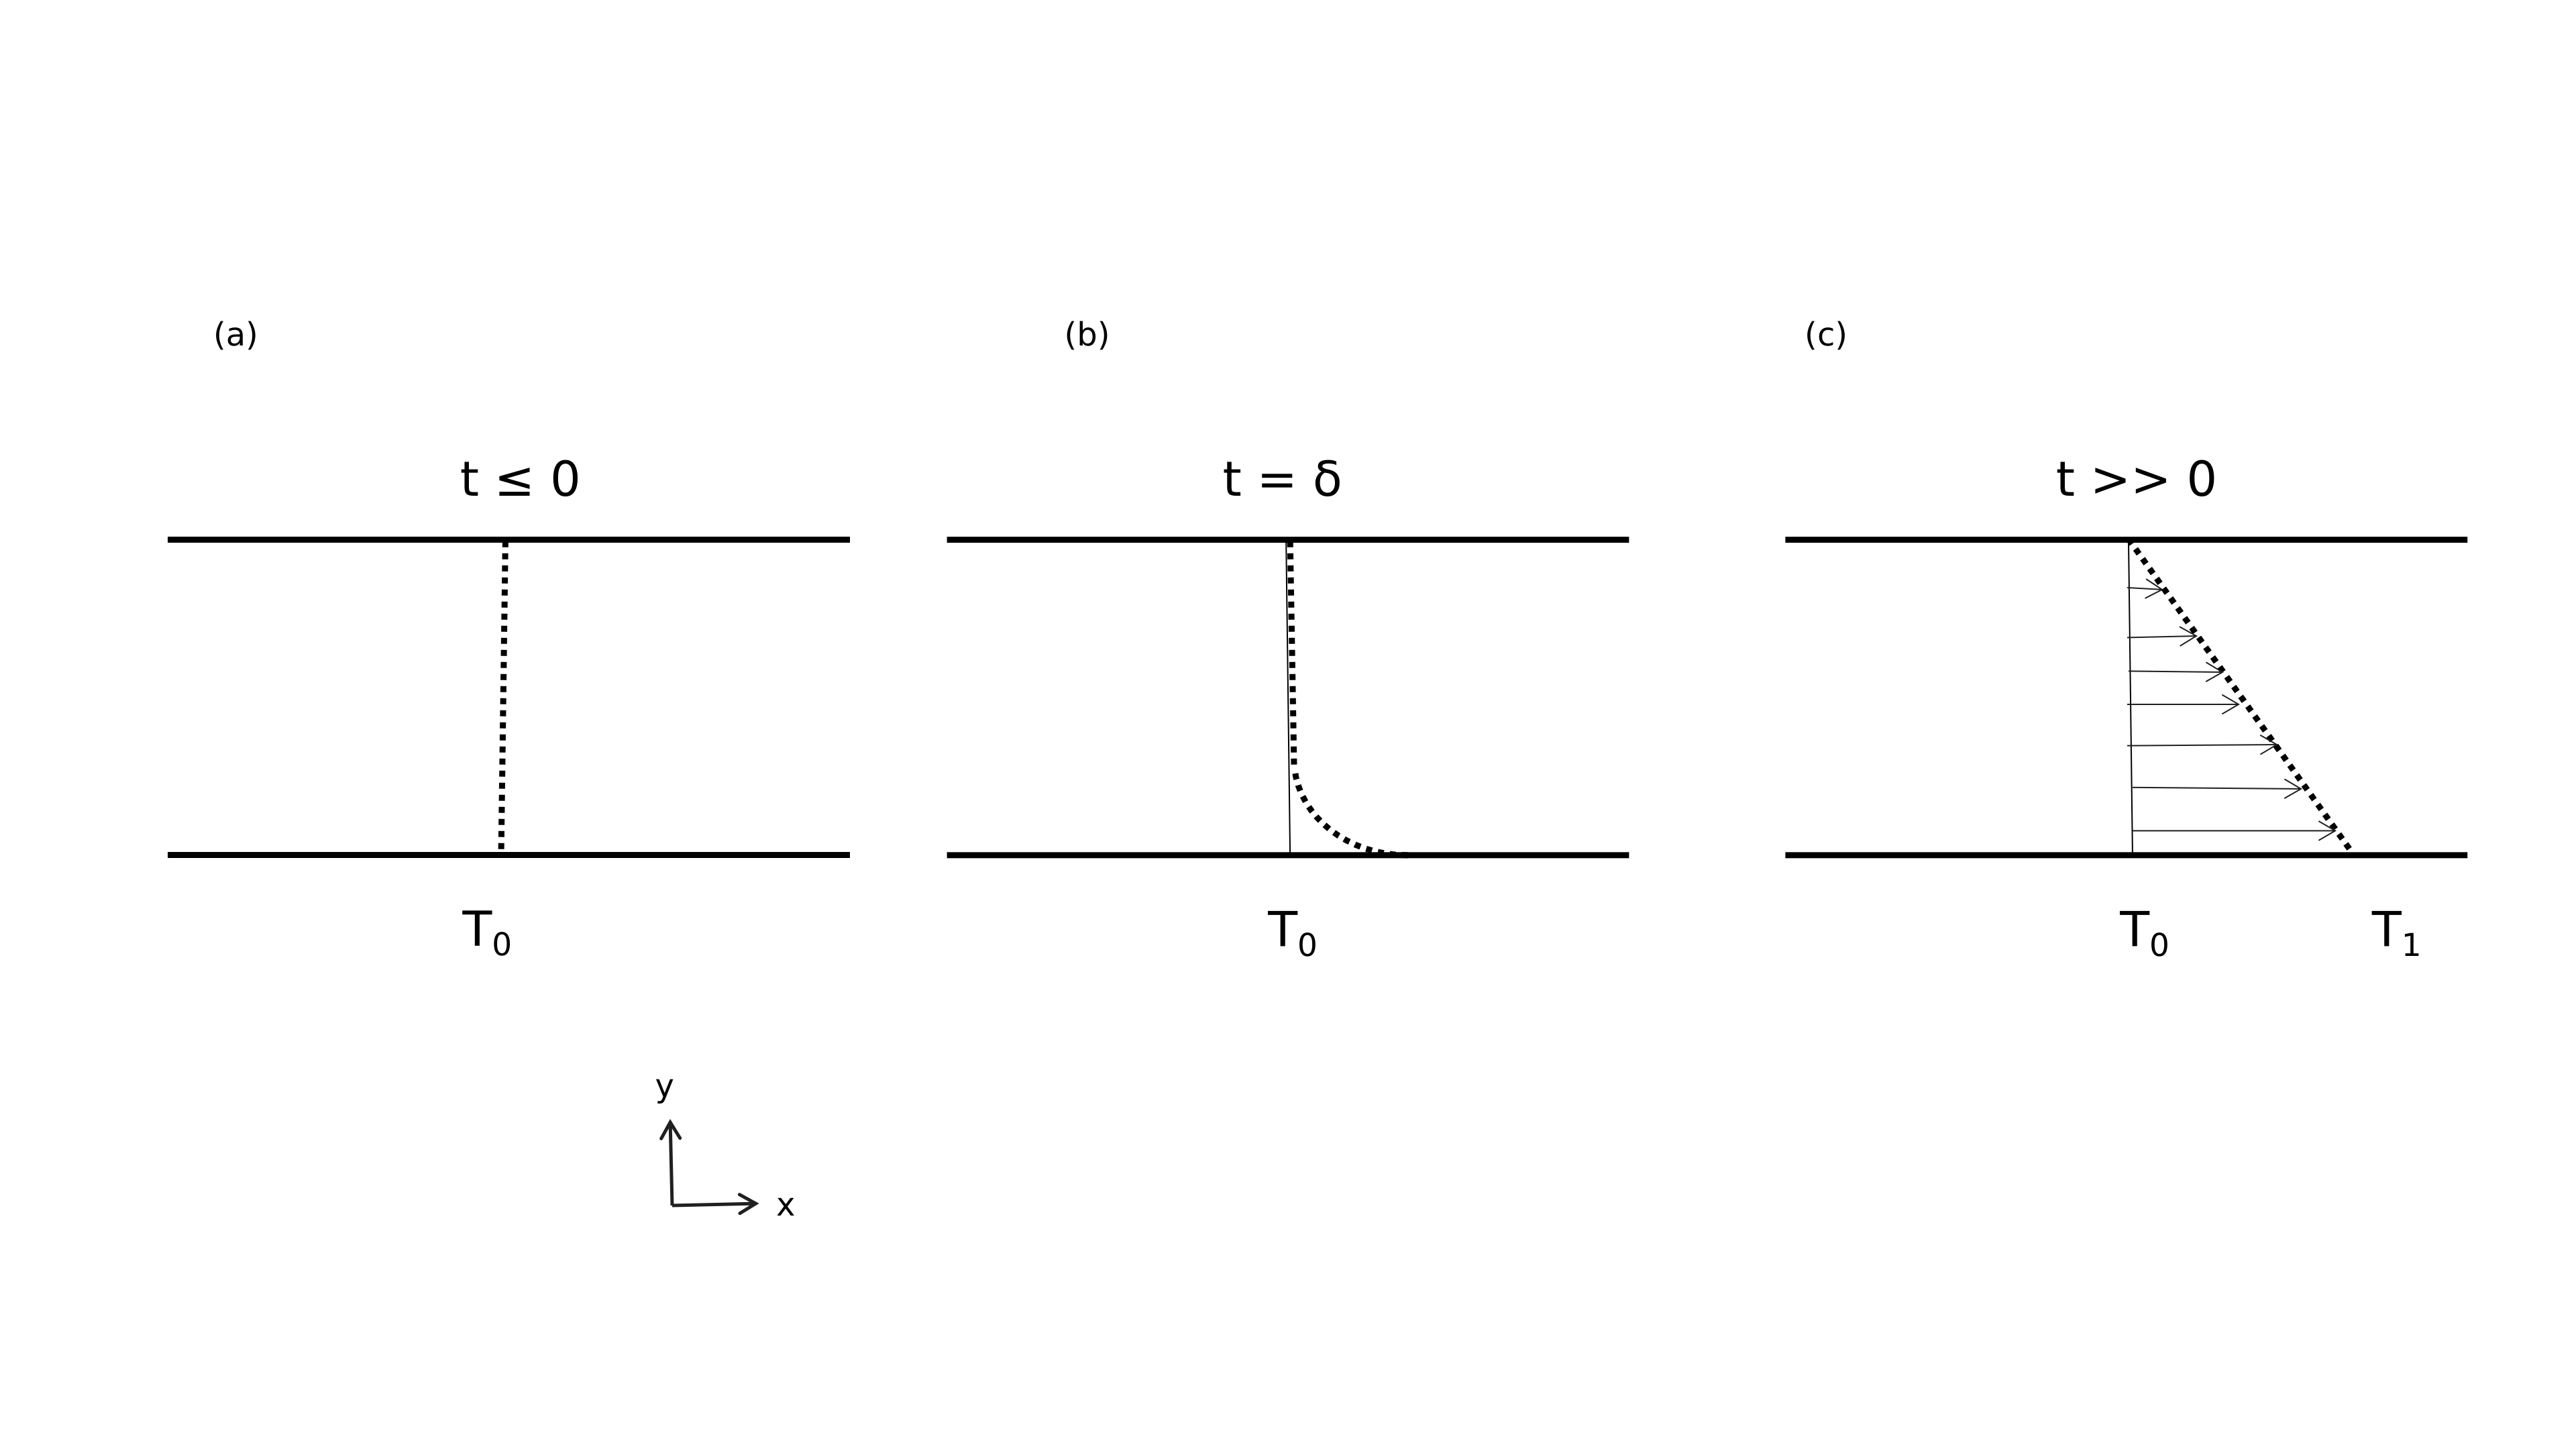
\includegraphics[scale=0.1]{figure1_02}
    \caption{Solid slab of conducting material between 2 plates}
\end{figure}

\begin{itemize}
    \item Consider two parallel plates : one placed at y = 0 and the other placed at y = Y as shown in figure 1.4, with a conducting solid between them. Here we assume these plates are basically infinitely long and wide. The system is at equilibrium withno heat sources anywhere. Figure 1.4(a) shows how the temperature is uniform at $T_{0}$ every point between the two plates. 

    \item Now, let us see what happens when we add a heat bath to the lower plate so that its temperature is kept at a slightly higher temperature $T_{1}$. If the temperature of the lower plate is uniformly at a temperature $T_{1}$ and is in contact with the solid material, two phenomena could occur to get energy across to atoms in the solid: 
        \SubItem{Either free electrons in the solid start to move quickly across it and hence transfer thermal energy}
        \SubItem{The periodic vibrations of atoms in the solid move across (phonon transport)}. 

    \item Figure 1.4(b) describes a snapshot of the system where some of the thermal energy has started to go across to the interface atoms of the slab but most of it is still yet unaffected.

    \item Note that the top plate is still exposed to the environment, which is assumed to be at the temperature $T_{0}$. Over time, the solid atoms begin to transmit heat across by the two mechanisms mentioned above and energy gets imparted along the y direction. Figure 1.4(c) showcases the steady-state temperature profile of the slab.
\end{itemize}

In the case of momentum transport, we computed the force needed to keep the lower plate moving at a velocity v. Here, the lower plate keeps transmitting its heat energy off to the slab. So how much heat does the heat bath need to supply to the lower plate to keep its temperature constant at $T_{1}$?

$$\frac{Q}{A} = k \frac{\Delta T}{Y}$$

It's a very similar expression to our initial expression for the force on a viscous liquid. This can similarly be extended to looking at the heat flux across every differential slice of the solid slab and hence we get the equation :

\begin{empheq}[box=\fbox]{align}
    q_{y} = -k \frac{dT}{dy}
\end{empheq}

This is called \textbf{Fourier's Law of Heat Conduction}. 

Some points to note :

\begin{itemize}

    \item Here, k is the thermal conductivity. It is a material property of the slab that describes the rate of heat conduction across it.
        
    \item Unlike fluid velocity, which is a vector, temperature is a scalar quantity. Similarly, in momentum transport, $\tau$ was a tensor. Here $q$ is a vector with components $q_{x}, q_{y}, q_{z}$ in directions perpendicular to the x, y and z axes. The multidimensional equivalent of Fourier's law is: $$q = -k \nabla T$$

    \item We have again made an implicit assumption that the thermal conductivity of the material is isotropic and that k is the same in all directions. In the case of fibrous materials and laminates, we can use the following equation : $$q = -\vec{\kappa} . \nabla T$$ where $\vec{\kappa}$ is a thermal conductivity tensor.


\end{itemize}

\subsection*{Some more points on thermal conductivity}

\begin{itemize}

    \item The thermal diffusivity of a system ($\alpha$) is the ratio of heat conducted to heat stored. It is given by the expression $$\alpha = \frac{k}{\rho C_{p}}$$ where $C_{p}$ is the heat capacity of the material

    \item There are two useful dimensionless constants in energy transport. The Prandtl number (Pr) given by : $$Pr = \frac{C_{p} \mu}{k}$$ and the Peclet number (Pe) given by $$Pe = Re Pr = \frac{d v}{\alpha}$$. 

\end{itemize}



\section{Mechanisms of Energy Transport}

There are three primary methods for energy transport that we are concerned with : \emph{Molecular Energy Transport} (which we have discussed thus far in the form of heat conduction), \emph{Convective energy transport} and \emph{Diffusive energy transport}. 


\subsection{Convective energy transport}

Convective energy transport is the energy transported by bulk movement of the fluid.

Consider a differential fluid element. The convective energy transport can be represented by $q^{(c)}$. It is again a vector with three components. Let the x-component be $q^{(c)}_{x}$. Here the surface of area dS is in a direction perpendicular to the x-axis as indicated in figure 1.5. The volume rate of flow across this surface is $v_{x} dS$. Now to get the total energy passing through this differential element, we need the energy per unit volume of the fluid flowing through, which is the sum of the kinetic energy per unit volume and the internal energy per unit volume. 


\begin{figure}[h]
    \centering
    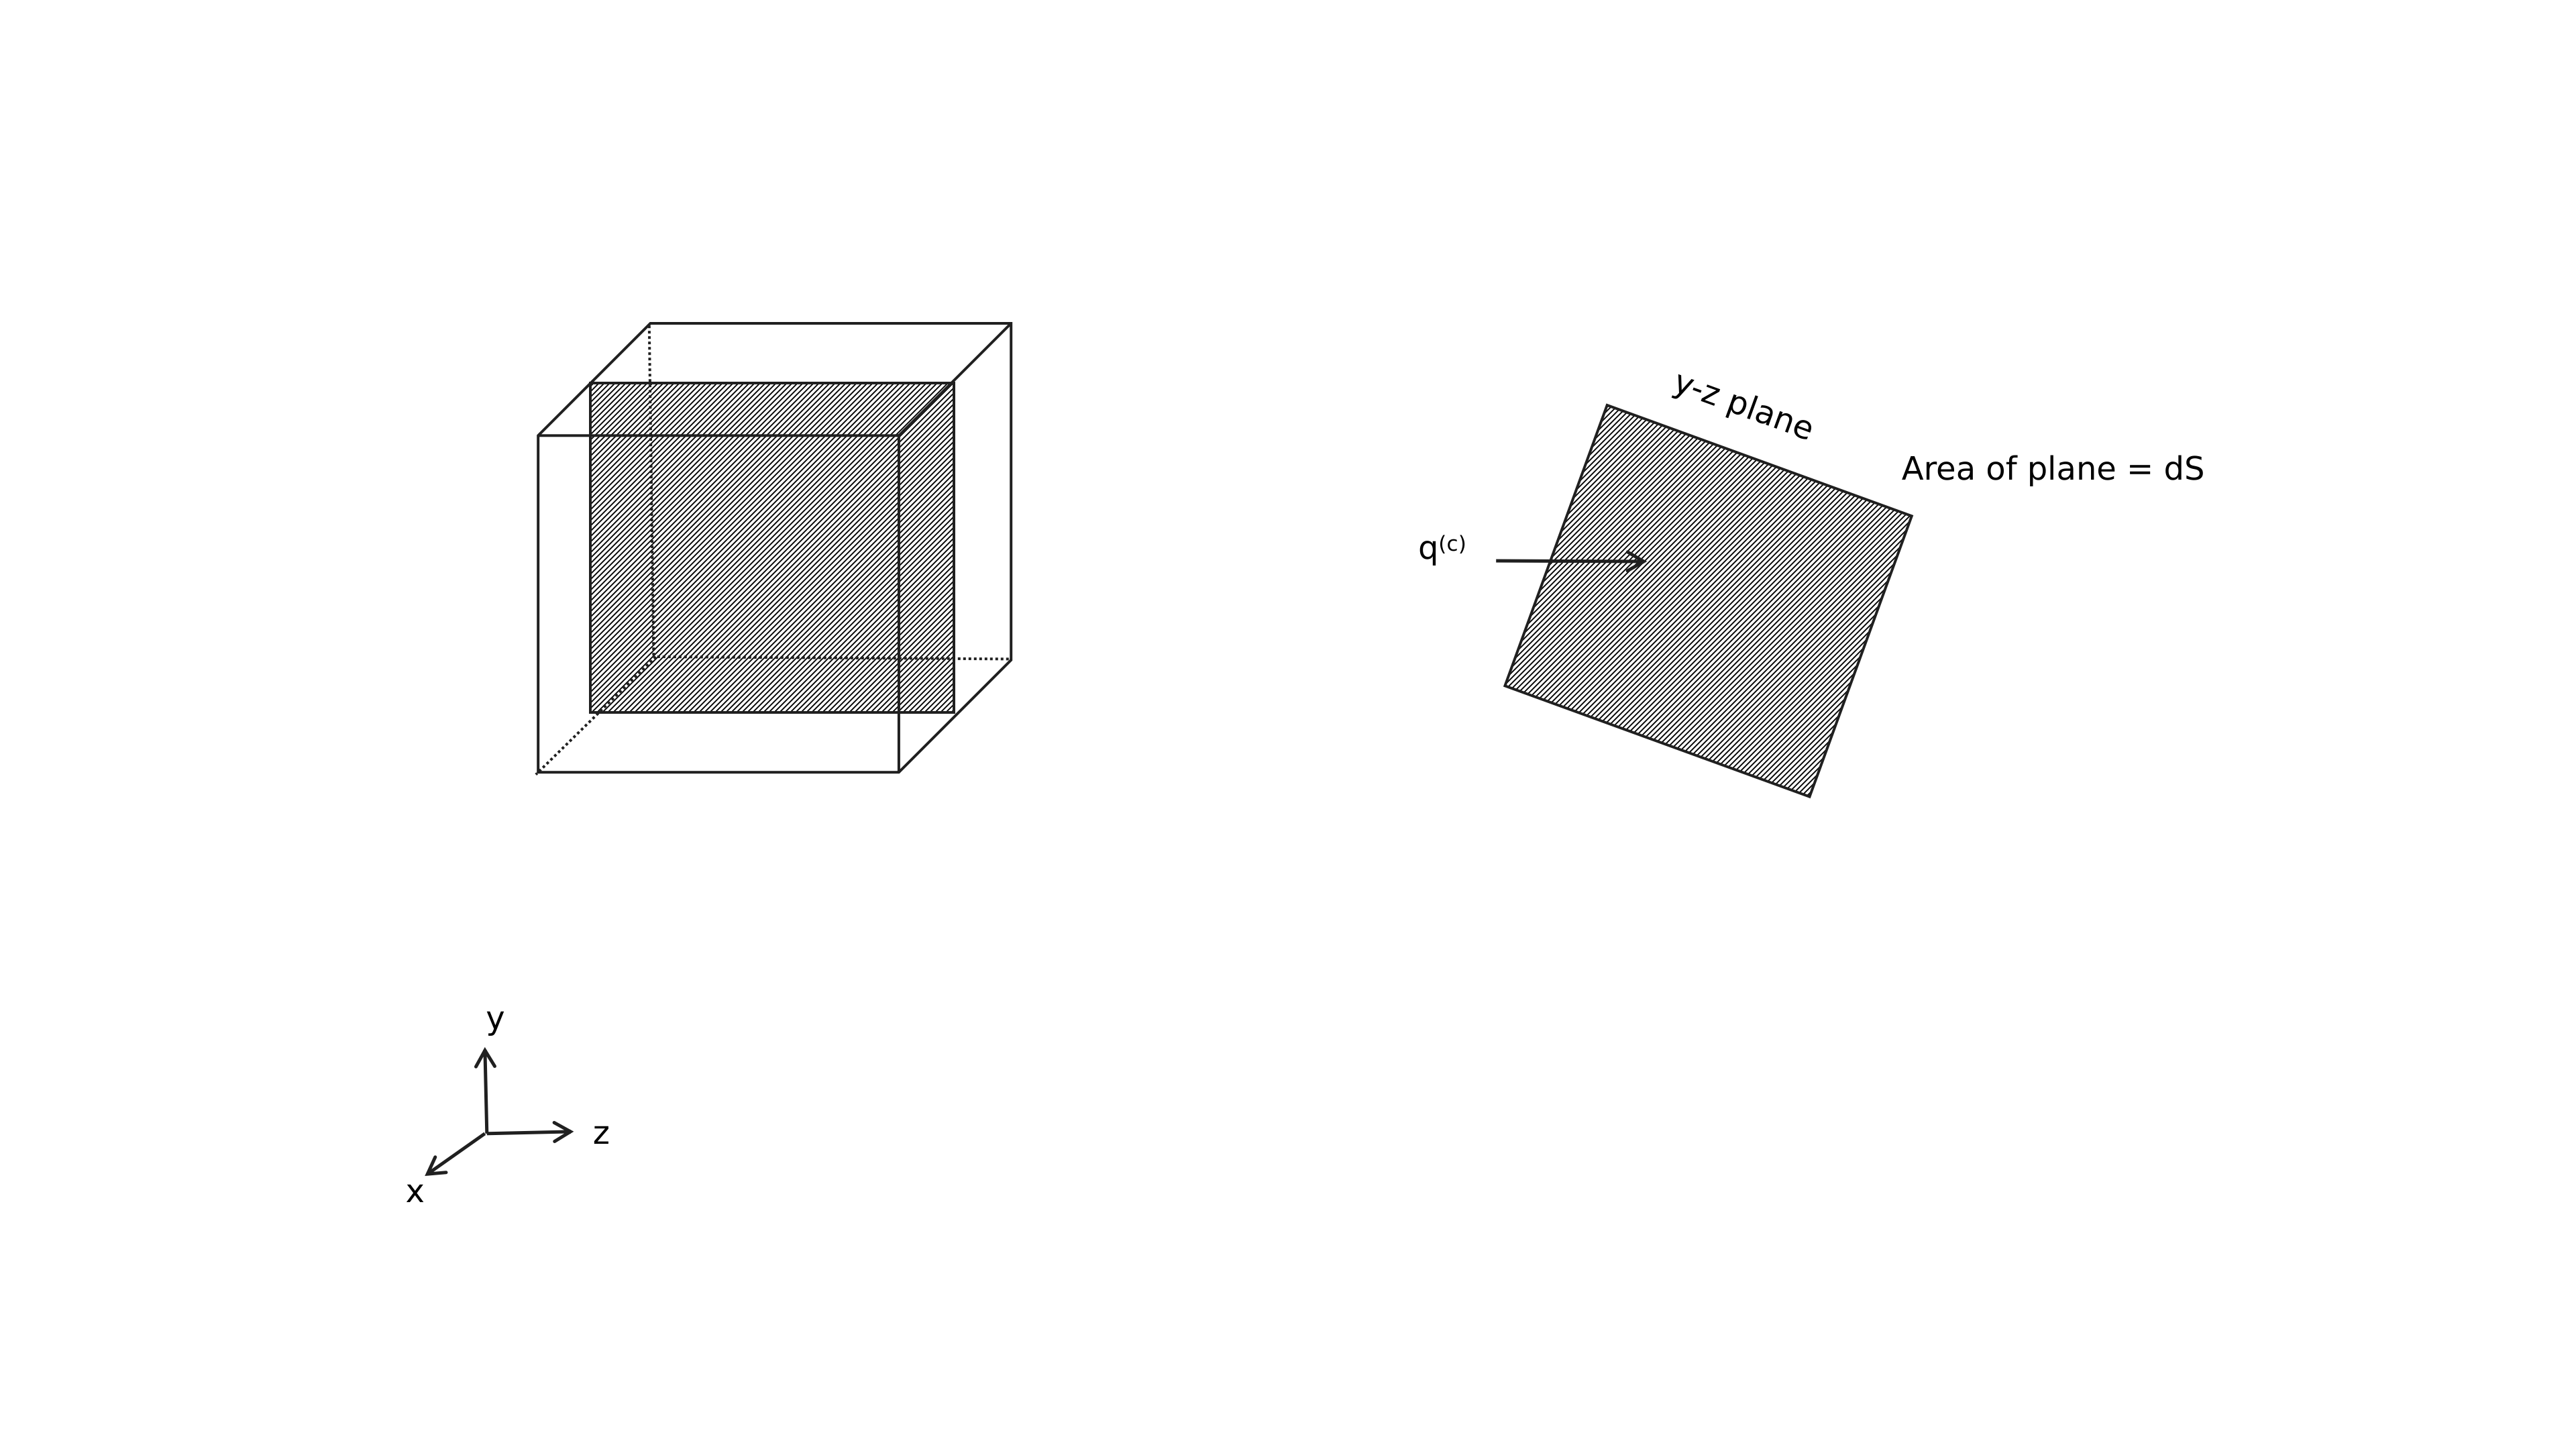
\includegraphics[scale=0.1]{figure2_03}
    \caption{Convective energy transport across a fluid element}
\end{figure}

$$q^{(c)}_{x} = (\frac{1}{2}\rho v^{2} + \rho U) v_{x} $$

Where, $v^{2} = v_{x}^{2} + v_{y}^{2} + v_{z}^{2}$. Representing this equation in general for the overall vector, we get:

\begin{empheq}[box=\fbox]{align}
    q^{(c)} = (\frac{1}{2} \rho v^{2} + \rho U) . \vec{v}
\end{empheq}

\subsection{Work associated with molecular motion}

Recall from the first law of thermodynamics that the change in internal energy for a closed system can be represented by the following equation:

$$dU = dq + dW$$

Hence for flow systems, we are yet to account for the work done by molecular motion of fluids. 

$$dW = F . dr$$

$$\frac{dW}{dt} = F . \frac{dr}{dt} = F . v$$

Since the forces appearing here are from molecular motion, we can use the molecular momentum flux to represent this force :

$$\frac{dW}{dt} = F . v = (\pi . dS) . v$$

Recall that the molecular momentum flux is given by $$\pi_{ij} = P \delta_{ij} + \tau_{ij}$$


\subsubsection*{Combined energy flux}

Similar to how we defined the combined momentum flux tensor for momentum transport, we have a helpful combined energy flux \emph{vector} (e) for energy transport.


\begin{empheq}[box=\fbox]{align}
    e = q + q^{(c)} + w
\end{empheq}

q is the Fourier's law conduction term. Expanding the second and third terms, $q^{(c)} = (\frac{1}{2} \rho v^{2} + \rho U)v$, $w = [\pi . v]$, giving us

$$e = q + (\frac{1}{2} \rho v^{2} + \rho U)v + [\pi . v]$$

Since $\pi = P \delta + \tau$, we can use the definition $H = U + PV$ from thermodynamics to construct an alternate equation for e, as such :

$$e = q + (\frac{1}{2} \rho v^{2} + \rho H)v + [\tau . v]$$

\section{Demonstrating Mass Transport}

\subsection{Diffusive Transport}

Let us once again revisit our example of a fluid between two surfaces. 

\begin{figure}[h]
    \centering
    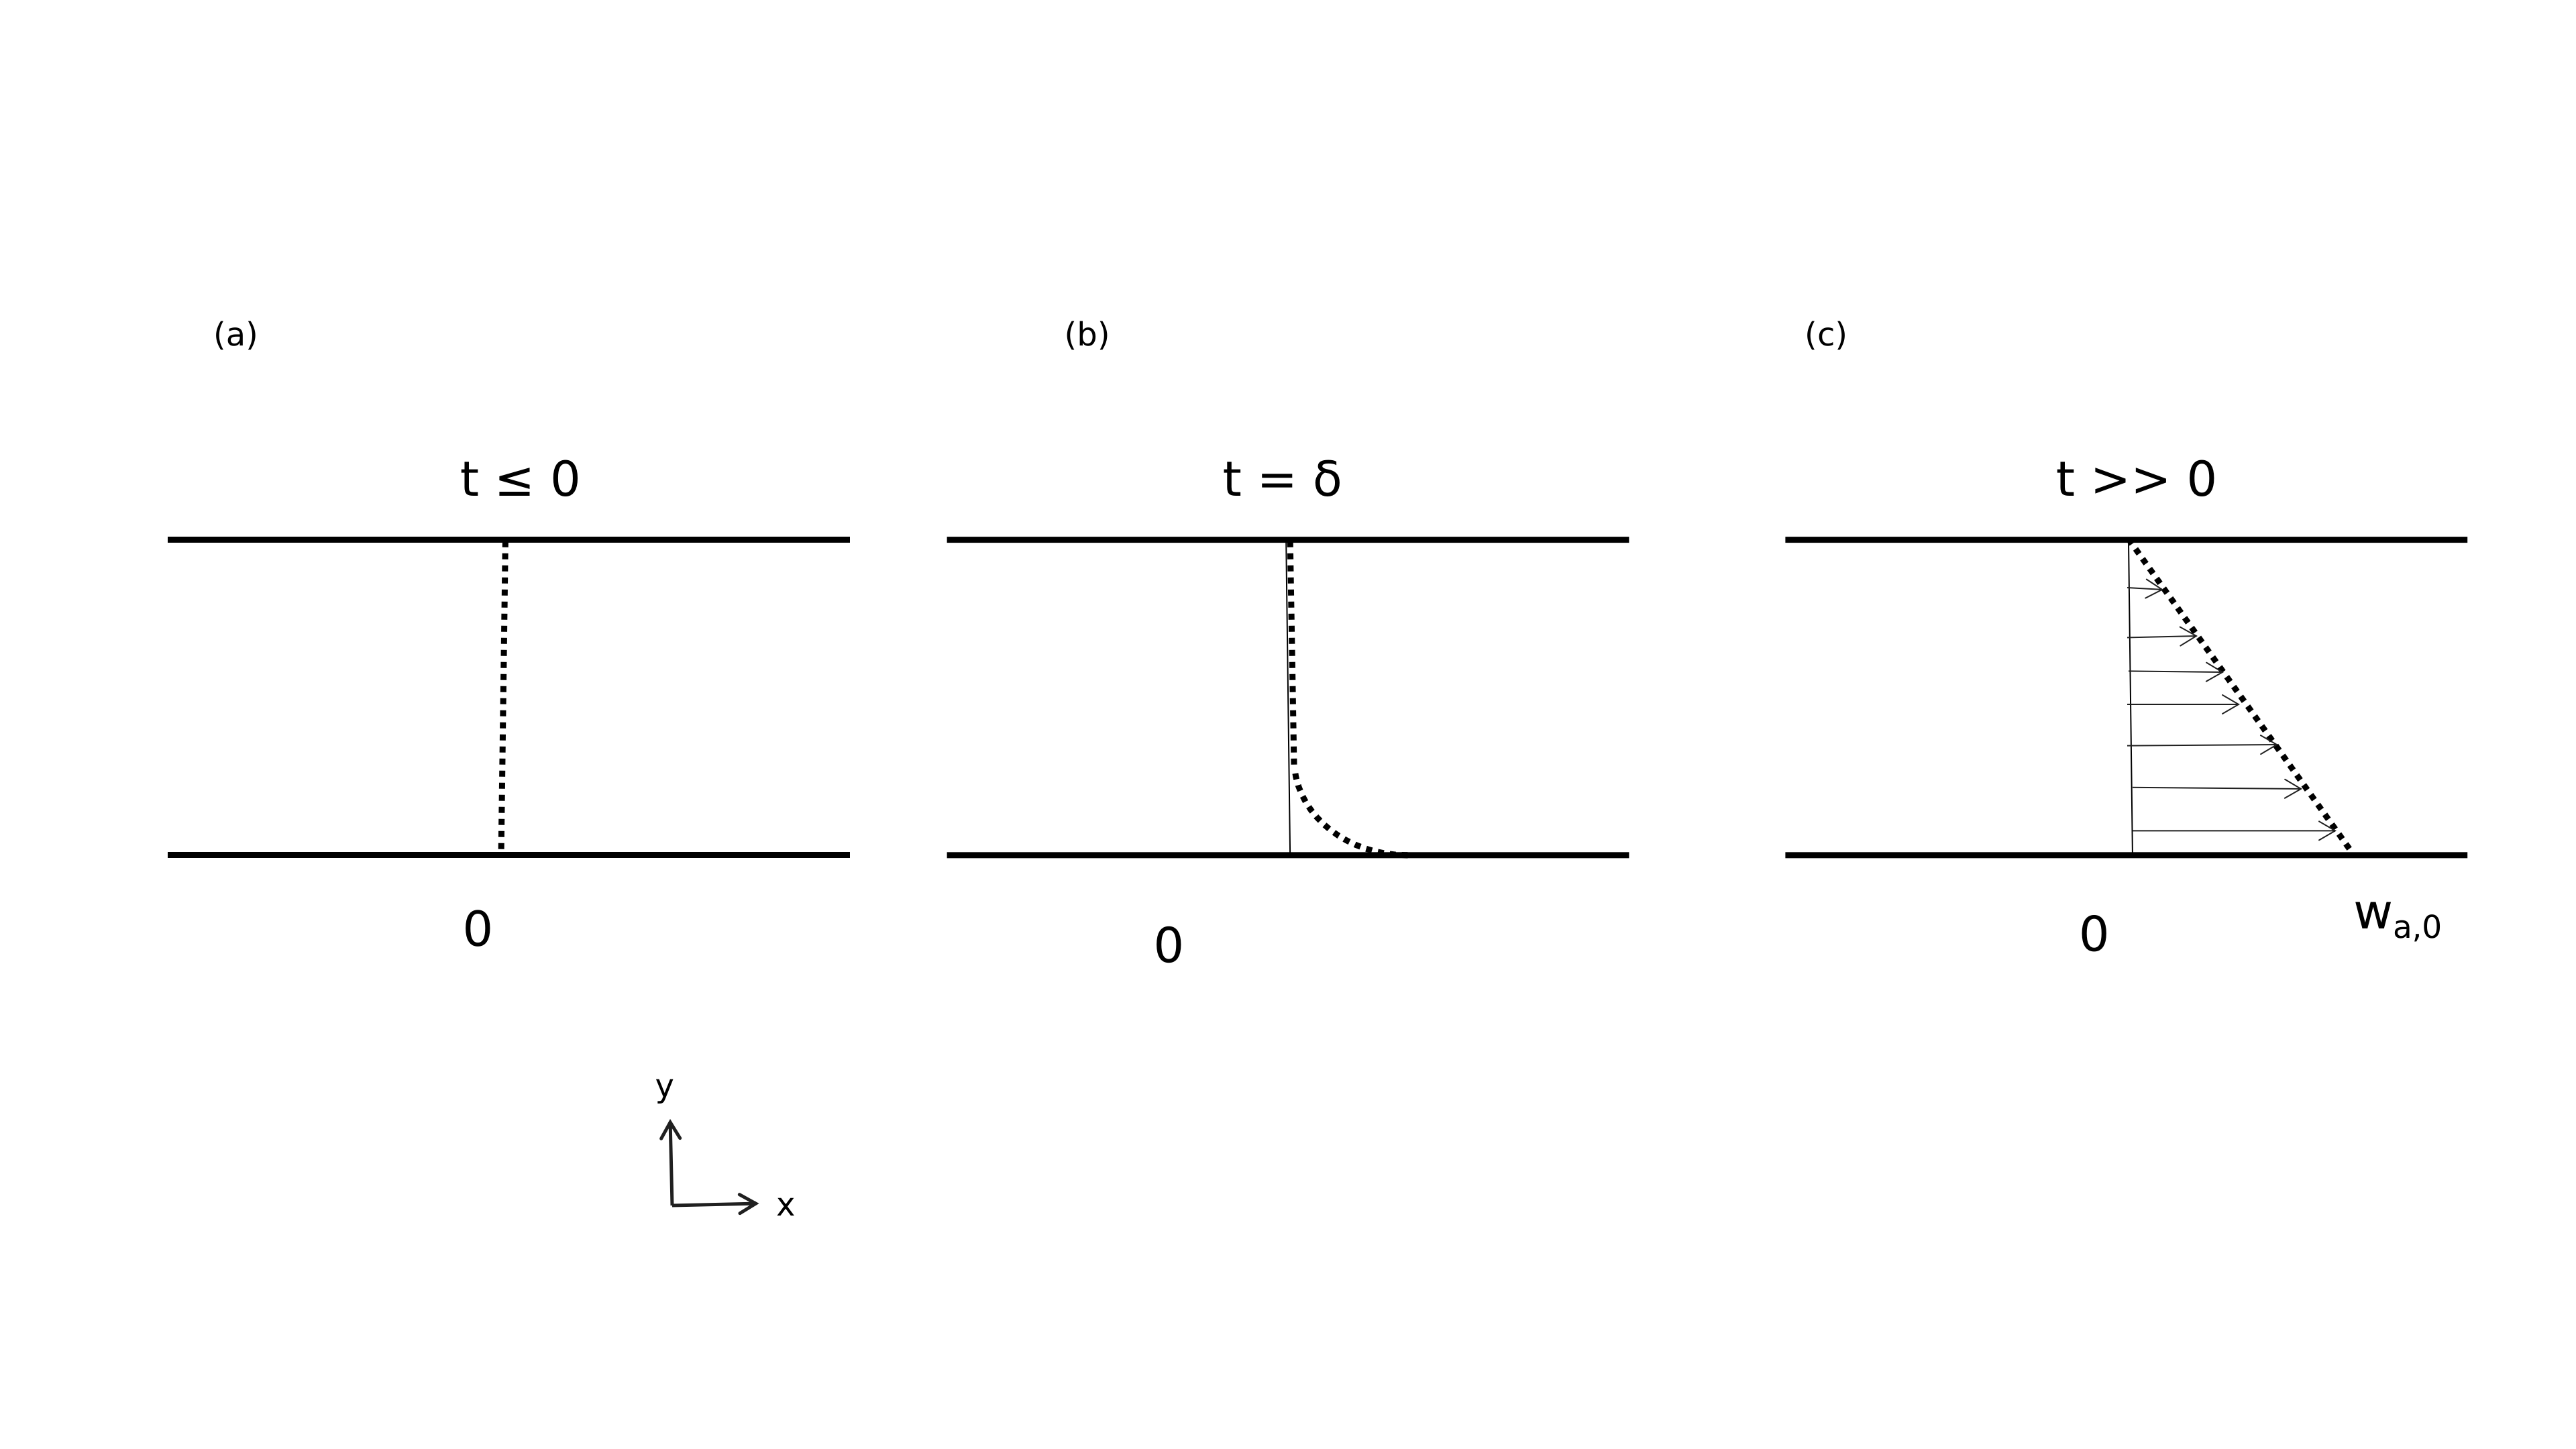
\includegraphics[scale=0.1]{figure1_03}
    \caption{Helium diffusion across a silica slab}
\end{figure}

\begin{itemize}
    \item Consider a silica slab. This silica slab can absorb helium, but not air. One end of this slab is at y = 0 and the other at y = Y as shown in figure 1.6. We are going to introduce some helium into this system eventually. We assume this slab is infinitely long and wide. The system is at equilibrium with air and there are no concentration gradients anywhere. Figure 1.6(a) shows how the concentration of helium is initially uniform at $0$ every point between the two ends of silica.
 
    \item Now, let us see what happens when we attach a helium source of concentration $w_{A0}$. The concentration of helium in the silica near the lower end is now $w_{A0}$. This helium starts to disperse across the silica elements near the bottom of the slab.

    \item Figure 1.4(b) describes a snapshot of the system where some of the helium has started to go across to the silica near the lower end of the slab.

    \item Note that the top end is still exposed to the environment where we just have air and the helium concentration is taken to be 0. Over time, the helium atoms begin to diffuse steadily across the slab and the concentration along points the y direction go up eventually. Figure 1.4(c) showcases the steady-state concentration profile of the slab.
\end{itemize}

The steady state concentration profile to a good approximation is given by the following expression:

$$\frac{w_{A}}{A} = \rho \mathscr{D}_{AB} \frac{w_{A0}}{Y}$$

Here $\mathscr{D}$ is the diffusivity. If we extend this to each differential slice across the slab:

\begin{empheq}[box=\fbox]{align}
    j_{Ay} = -\rho \mathscr{D}_{AB} \frac{dw_{A}}{dy}
\end{empheq}

Here, $j_{Ay}$ is the mass flux.

This is called \textbf{Fick's Law of Diffusion}.

Some points to note :

\begin{itemize}

    \item Here, $\mathscr{D}$ is the diffusivity. We write $\mathscr{D}_{AB}$ to indicate that we are describing the diffusivity of component A across a medium B.

    \item Unlike fluid velocity, which is a vector, concentration is a scalar quantity. Similarly, in momentum transport, $\tau$ was a tensor. Here $j_{A}$ is a vector with components $j_{Ax}, j_{Ay}, j_{Az}$. These are mass fluxes in the directions perpendicular to the x, y and z axes. The multidimensional equivalent of Fourier's law is: $$j_{A} = -\rho \mathscr{D}_{AB} \nabla w_{A}$$

\end{itemize}

\subsection{Convective mass transport}

As discussed before, transport can also occur with bulk fluid motions. Here let's look at mass transport for bulk fluid motions. Across a fluid element, let us think of the mass transport across a plane perpendicular to the x-axis (or parallel to the yz plane). 

\begin{figure}[h]
    \centering
    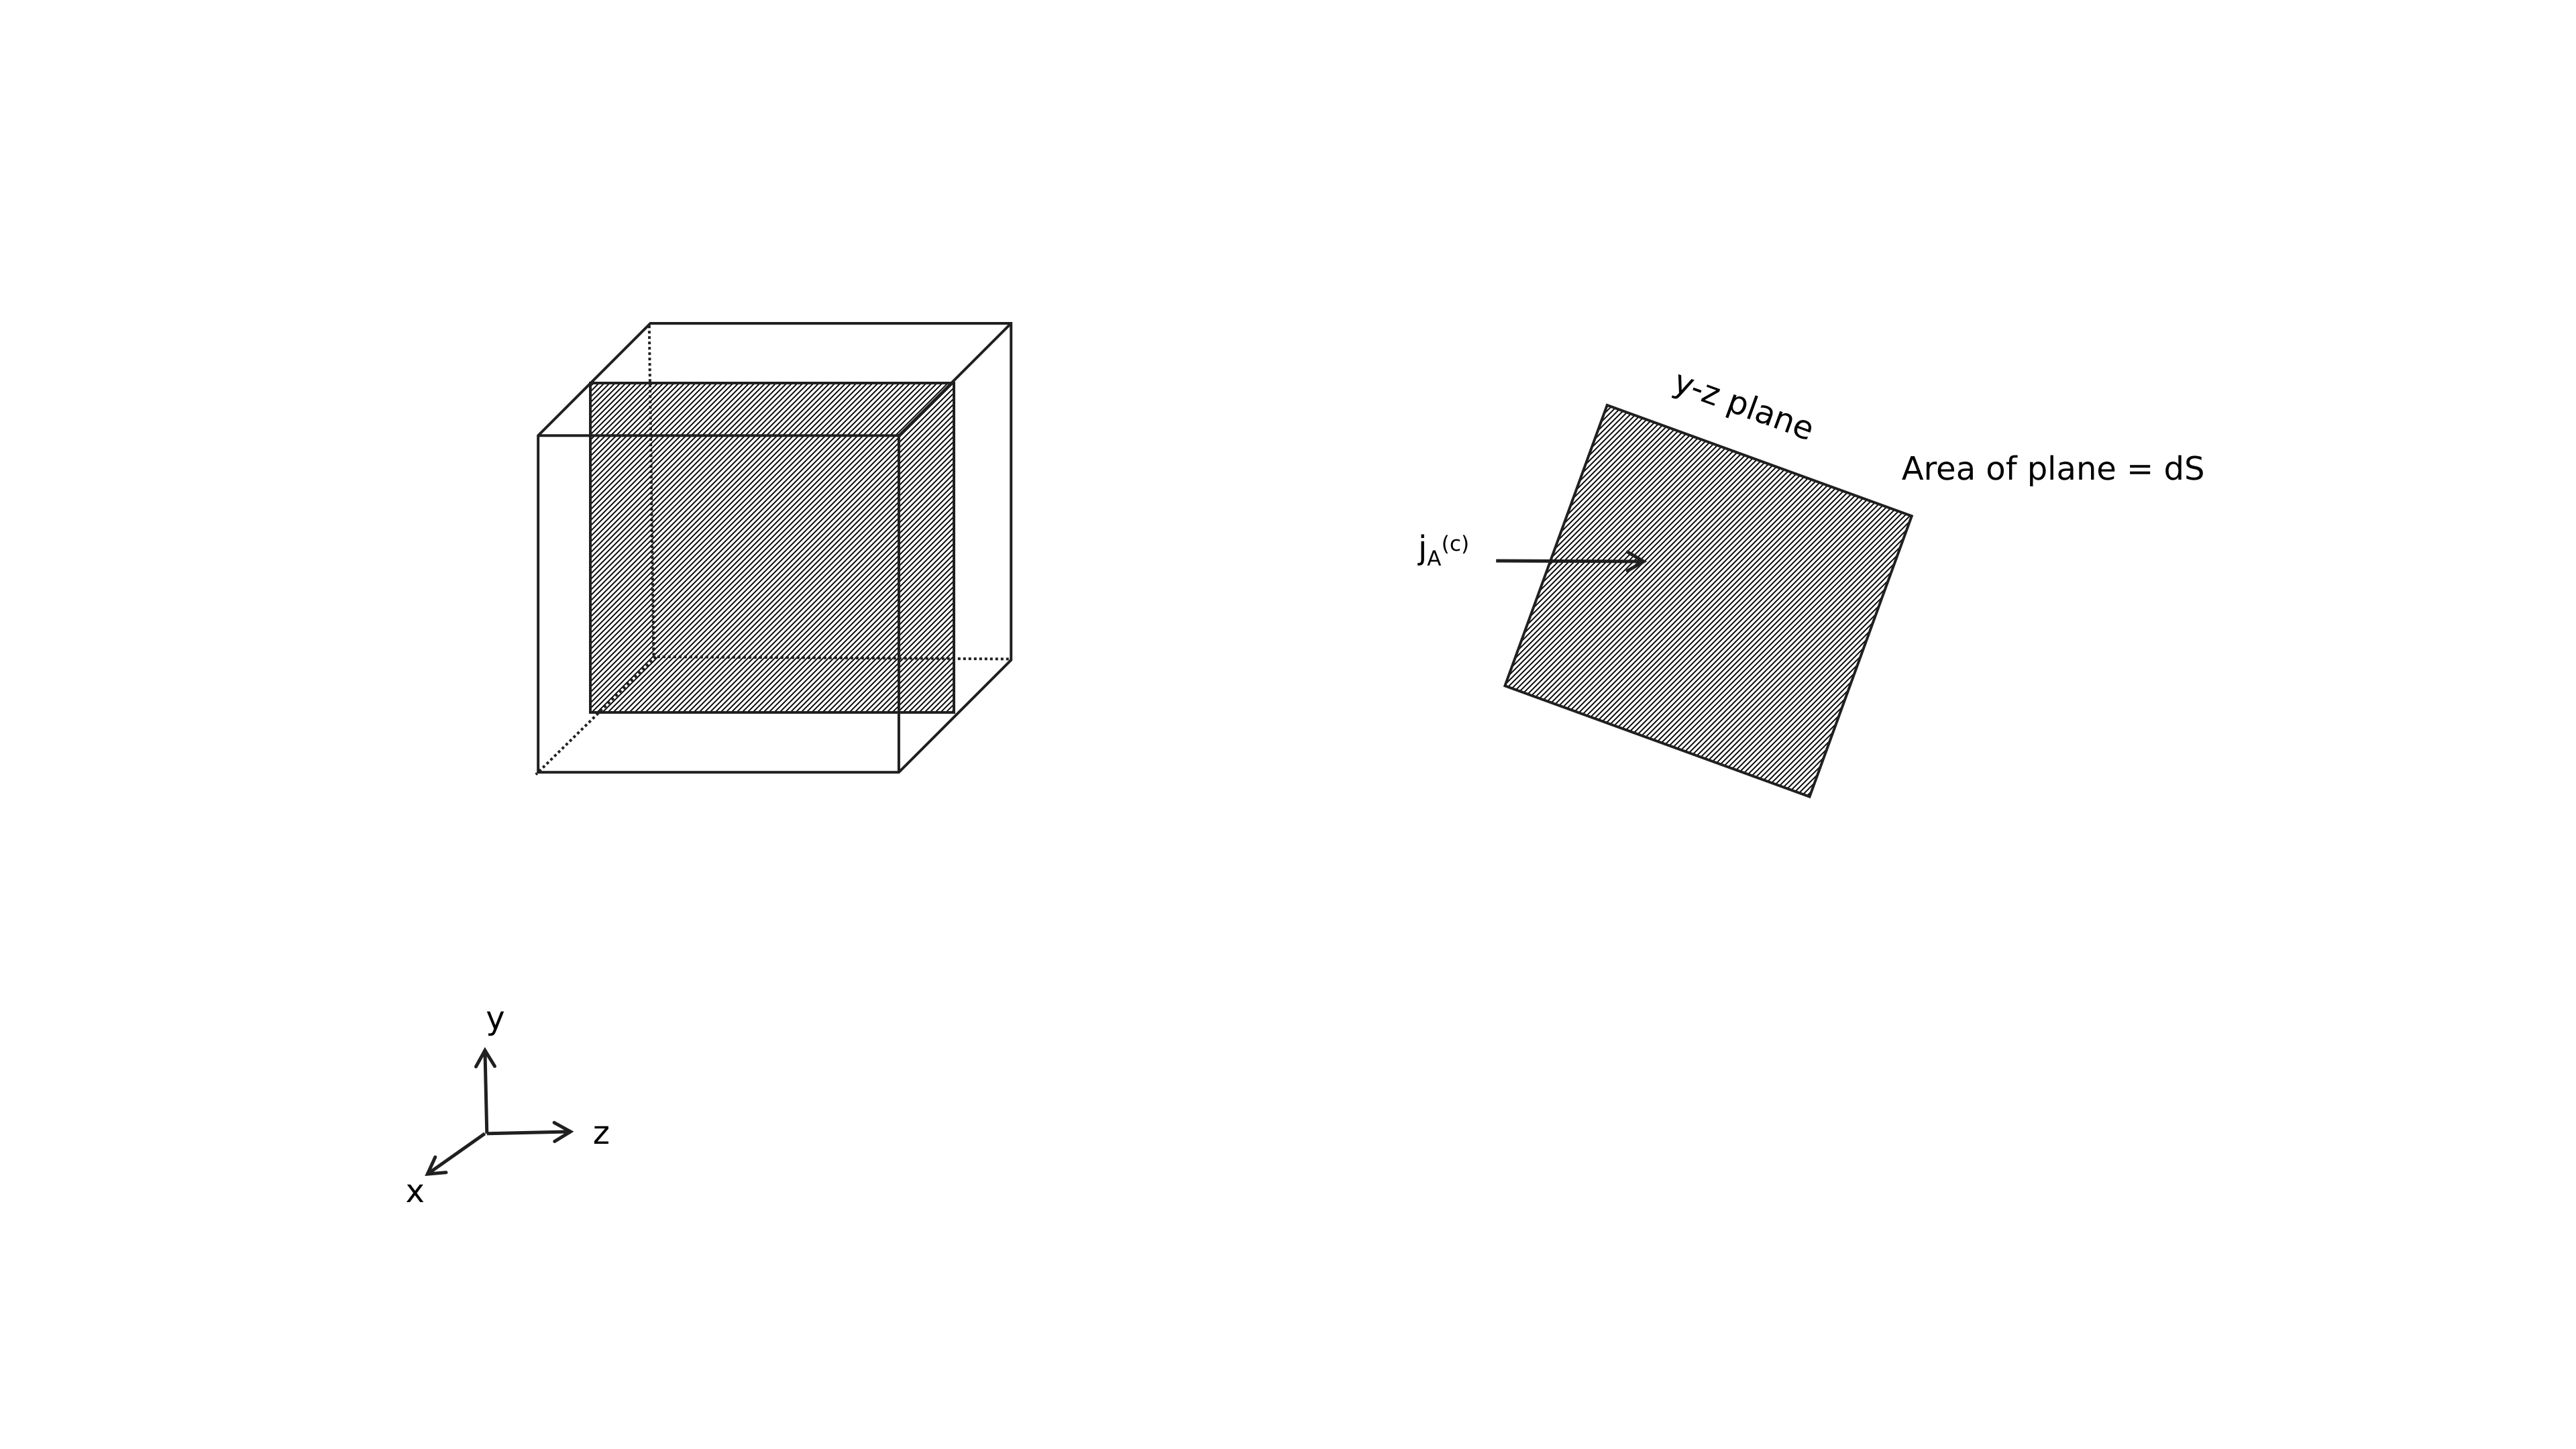
\includegraphics[scale=0.1]{figure2_04}
    \caption{Convective mass transport across an element}
\end{figure}

Let the convective mass transport be given by $j_{A}^{(c)}$. The mass per unit volume is the density $\rho_{A}$ of component A. The x-component of convective mass flux is hence given by $j_{Ax}^{(c)} = \rho_{A} v_{x} dS$. In three dimensions this is $j_{A}^{(c)} = \rho_{A} \vec{v}$

\subsection{Notation in mass transport}

Since there are various ways of denoting concentration, velocity and flux in mass transport, it is important to have a glossary of all the notation. 

Note that we will only be covering binary (or 2-component) systems here as the discussion of multi-component systems is very tricky and involves complicated expressions.

Some of the important equations and definitions you need to remember as follows:

\begin{itemize}
    \item $\rho_{A}$ is the mass of A per unit volume.
    \item $\rho = \rho_{A} + \rho_{B}$ is the mass density of the fluid mixture.
    \item $w_{A} = \frac{\rho_{A}}{\rho}$ is the mass fraction of A in the mixture.
    \item $w_{A} + w_{B} = 1$. Which means that $\nabla w_{A} = - \nabla w_{B}$.
    \item $c_{A}$ is the number of moles of A per unit volume.
    \item $c = c_{A} + c_{B}$ represents the total molar concentration.
    \item $x_{A} = \frac{c_{A}}{c}$ is the mole fraction of A in the mixture.
    \item $x_{A} + x_{B} = 1$, which again means that $\nabla x_{A} = - \nabla x_{B}$.
    \item $\rho = cM$ where M is the molecular weight. This means that $w_{A} = \frac{x_{A} M_{A}}{M}$
    \item $\nabla w_{A} = \frac{M_{A} M_{B} \nabla x_{A}}{M^{2}} = \frac{w_{A} w_{B} \nabla x_{A}}{x_{A} x_{B}}$. This helps in converting representations of mass concentrations to molar concentrations and vice versa. 
    \item $v_{A}$ is the velocity of component A.
    \item The mass-average velocity v is given by $v = \frac{\rho_{A} v_{A} + \rho_{B} v_{B}}{\rho_{A} + \rho_{B}}$ = $w_{A} v_{A} + w_{B} v_{B}$.
    \item The convective mass flux vector is given by $j_{A}^{(c)} = \rho_{A} v$.
    \item The molar-average velocity $v^{*}$ is given by $v^{*} = x_{A} v_{A} + x_{B} v_{B}$.
    \item The convective molar flux vector is given by $J_{A}^{(c)} = c_{A} v^{*}$
    \item Fick's law in terms of mass-flux vector : $j_{Ay} = -\rho_{A} \mathscr{D}_{AB} \frac{dw_{A}}{dy}$.
    \item Fick's law in terms of molar-flux vector : $J_{Ay}^{*} = -c \mathscr{D}_{AB} \frac{dx_{A}}{dy}$.
\end{itemize}

\subsubsection*{Useful Dimensionless Groups in Mass Transport}

\begin{itemize}

    \item Prandtl Number $Pr = \frac{\nu}{\alpha} = \frac{C_{p} \mu}{k}$

    \item Schmidt Number $Sc = \frac{\nu}{\mathscr{D}_{AB}} = \frac{\mu}{\rho \mathscr{D}_{AB}}$
        
    \item Lewis Number $Le = \frac{\alpha}{\mathscr{D}_{AB}} = \frac{k}{\rho C_{p} \mathscr{D}_{AB}}$.

\end{itemize}

\subsubsection*{Combined flux vectors in mass transport}

The combined mass-flux vector $n_{A}$ is given by:

$$n_{A} = j_{A}^{(c)} + j_{A} = \rho_{A} v - \rho \mathscr{D}_{AB} \nabla w_{A}$$

The combined molar-flux vector $N_{A}$ is given by:

$$N_{A} = J_{A}^{* (c)} + J_{A}^{*} = c_{A} v^{*} - c \mathscr{D}_{AB} \nabla x_{A}$$

For binary mixtures, the most useful expressions that can be used for the mass-flux and molar-flux vectors are:


\begin{empheq}[box=\fbox]{align}
    n_{A} = w_{A} (n_{A} + n_{B}) - \rho \mathscr{D}_{AB} \nabla w_{A} \\
    N_{A} = x_{A} (N_{A} + N_{B}) - \rho \mathscr{D}_{AB} \nabla x_{A}
\end{empheq}




